\documentclass[smaller]{beamer}
\usepackage[english]{babel}
\usepackage[utf8]{inputenc}
\usepackage{graphicx}
\usepackage{multimedia, tikz}
\usetikzlibrary{decorations.fractals}
\usepackage{amsmath,amsthm,amssymb}
\usepackage{mathrsfs}

\usetheme{Singapore}
\setbeamertemplate{blocks}[rounded][shadow=true]
\setbeamercolor{block title}{bg=gray!10}
\setbeamercovered{transparent}

\title{Fractal Growth}
\subtitle{Seminar on Computational Physics}
\author{Benedikt Sauer, Alexander Schroer}
\institute{HISKP\\Universität Bonn}
\date{2$^\mathsf{nd}$ March 2011}

\begin{document}

    \begin{frame}
        \titlepage
    \end{frame}
    
    \begin{frame}
        \begin{center}
            \only<1>{\includegraphics[width=7cm]{img/intro_01.png}}
            \only<2>{\includegraphics[width=7cm]{img/intro_02.png}}
            \only<3>{\includegraphics[width=7cm]{img/intro_03.png}}
            \only<4>{\includegraphics[width=7cm]{img/intro_04.png}}
            \only<5>
            {
                \includegraphics[width=7cm]{img/intro_05.png}

                \color{gray}T. A. Witten, L. M. Sander, 1981
            }
        \end{center}
    \end{frame}

    \begin{frame}{Outline}
        \tableofcontents
    \end{frame}

    \section{Mathematical introduction}
        \subsection{Definitions and examples}
                \begin{frame}{Fractal Dimension}
                    \begin{definition}[Hausdorff measure]
                      The (outer) $d$-dimensional Hausdorff measure is defined as:
                      \begin{align}
                        H^d_\varepsilon(S)=
                        \inf_{\substack{\bigcup_{i=1}^\infty U_i\supset S\\ \operatorname{diam}(U_i) <
                        \varepsilon}}
                            \sum_{i=1}^\infty \operatorname{diam}(U_i)^d
                      \end{align}
                      The $d$-dimensional measure is (modulo some measure theory) the limit
                      $\varepsilon \to 0$. \pause
                    \end{definition}

                      \begin{definition}[Hausdorff dimension]
                        The Hausdorff dimension of a set is defined as:
                        \begin{align}
                          d_H = \sup\{d\in\mathbb{R}^+_0\ |\ H^d(S) = \infty\}
                        \end{align}
                      \end{definition}
                \end{frame}

        \subsection{Fractal dimension of discretized, finite structures}
                \begin{frame}{Discrete Calculations}
                  \begin{definition}[Simpler working definition]
                    The fractal dimension of a point set is defined as the following:
        
                    $$D=-\lim_{R\rightarrow 0}\frac{\log(N)}{\log(R)}$$

                  \end{definition} \pause

                  \begin{center}
                  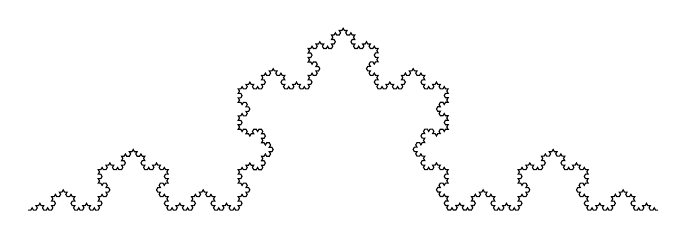
\begin{tikzpicture}[decoration=Koch snowflake]
                    \draw decorate 
                          { decorate { decorate { decorate { decorate {
                          (0,0) -- (8,0) }}}}};
                  \end{tikzpicture}
                \end{center}
                \end{frame}

            \begin{frame}{Fractal dimension of finite structures}
                \begin{columns}
                    \begin{column}{6cm}
                        \includegraphics[width=6cm]{img/frac_01.png}
                    \end{column}
                    \begin{column}{5cm}
                        Box-counting:
                        $\log(N)=-d \log(\epsilon)$

                        \vspace{1cm}
                        Other scaling power-laws:
                        \begin{itemize}
                            \item radius of gyration $R_g\propto N^{1/d}$
                            \item density-density-correlation $C(r)\propto r^{D-d}$
                            \item ...
                        \end{itemize}
                    \end{column}
                \end{columns}
            \end{frame}

    \section{Basic models}
        \subsection{Diffusion/number limited growth}
            \begin{frame}{The Meakin model}
                \begin{center}
                    \begin{columns}
                        \begin{column}{7cm}
  \begin{enumerate}
    \item \begin{itemize}
            \item Set seed in the center of the lattice
            \item Generate particles at $R+10$ one by one
            \item Let particle diffuse against the cluster
            \item Particles further than $2R$ are removed
          \end{itemize}
\pause
\vspace{1cm}
    \item \begin{itemize}
            \item Generate many particles once
            \item Let them diffuse and clump together
            \item Steady state is reached
          \end{itemize}
  \end{enumerate}
                        \end{column}
                        \begin{column}{3cm}
                            \includegraphics[width=3.0cm]{img/meakin_01.png}
                        \end{column}
                    \end{columns}
                \end{center}
            \end{frame}
\begin{frame}{Implementation: Outline}
  Two types of objects:
  \begin{itemize}
    \item Particles (which carry interaction information) \pause
    \item Clusters (specialized containers for particles) \pause
  \end{itemize}\pause
  \vspace{0.3cm}
  The main program step works as follows:
  \begin{itemize}
    \item Update the environment \pause
      \begin{itemize}
        \item Remove particles that are too far away or to old
        \item Create new particles or clusters
      \end{itemize} \pause
    \item Let particles and clusters interact \pause
      \begin{itemize}
        \item If they are near enough merge them
        \item Else let them move randomly \pause
          by probabilities calculated in the interaction
      \end{itemize}
  \end{itemize} \pause
  If we want we output graphics or calculate statistics afterwards.
\end{frame}


            \begin{frame}{Fractal dimension of 2-d Meakin clusters}
                \includegraphics[width=10cm]{img/meakin_02.jpg}
            \end{frame}

            \begin{frame}{Fractal dimension of 3-d Meakin clusters}
                \includegraphics[width=10cm]{img/meakin_03.jpg}
            \end{frame}

            \begin{frame}{Anaglyph of 3-d Meakin cluster (8000 particles)}
                \begin{center}
                    \includegraphics[width=8cm]{img/meakin_04.png}
                \end{center}
            \end{frame}

    \section{Towards application}
        \subsection{Encouraged self-similar growth}
            \begin{frame}{Encouraged self-similar growth}
                \begin{center}
                    \begin{itemize}
                        \item Want to create structures with tailor-made dimensionality while maintaining basic building principle (physically motivated!)
                        \item Idea: Encourage certain scaling behaviour (remember $D\approx -\frac{\log{N}}{\log{\epsilon}}$)
                        \item Diffuse clusters instead of particles
                    \end{itemize}

                    \vspace{.5cm}
                    \includegraphics[width=10cm]{img/self-sim_01.png}
                \end{center}
            \end{frame}           

            \begin{frame}
                A theoretical treatment is difficult:
                \begin{itemize}
                    \item Hybridization of IFS and statistical process, so no simple scaling law
                    \item Non-negligible finite-size effects
                \end{itemize}

                \begin{center}
                    \includegraphics[width=7cm]{img/self-sim_02.jpg}
                \end{center}
            \end{frame}

        \subsection{Dendrites}
            \begin{frame}{Dendrites}
               \begin{columns}
                    \begin{column}{6cm}
                        \includegraphics[width=6cm]{img/dendrite_01.png}
                    \end{column}
                    \begin{column}{6cm}
                        \includegraphics[width=6cm]{img/dendrite_02.png}
                    \end{column}
               \end{columns} 
            \end{frame}

        \subsection{Tubes}
            \begin{frame}{Tubes}
                \begin{columns}
                    \begin{column}{5cm}
                        \includegraphics[width=5cm]{img/tube_03.png}
                    \end{column}
                    \begin{column}{5cm}
                        \includegraphics[width=5cm]{img/tube_01.png}
                    \end{column}
               \end{columns} 
            \end{frame}

            \begin{frame}{Tubes: flux}
                \begin{center}
                    \includegraphics[width=10cm]{img/tube_02.png}
                \end{center}
            \end{frame}

            \begin{frame}{Tubes: flux}
                \begin{center}
                    \includegraphics[width=8cm]{img/tube_04.jpg}

                    \color{gray}
                    2-dimensional simulation, length/radius: 10
                \end{center}
            \end{frame}

            \begin{frame}{Tubes: real-world physics?}
                \begin{columns}
                    \begin{column}{5cm}
                        Obstacles are fixed unphysically:
                        \begin{itemize}
                            \item require breaking of bonds
                            \item leads to MD-like simulations
                        \end{itemize}
                    \end{column}
                    \begin{column}{5cm}
                        \includegraphics[width=5cm]{img/tube_05.png}
                    \end{column}
               \end{columns} 
            \end{frame}

        \subsection{Crystalization}
            \begin{frame}{Crystals vs. Dendrites}
                \begin{center}
                    \begin{columns}
                        \begin{column}{5.5cm}
                            Idea: Add Coulomb-like interaction
                            \begin{itemize}
                                \item Introduce particle charge
                                \item Set preferred directions in random walk depending on other particles
                                \item Try to observe a transition from $D=1.6$ to $D=2$
                            \end{itemize}
        
                            This is work in progress.
                        \end{column}
                        \begin{column}{5cm}
                            \includegraphics[width=4.5cm]{img/coulomb_01.png}
                        \end{column}
                    \end{columns}
                \end{center}
            \end{frame}

    \section{An organic model}
        \subsection{Tumor growth}
            \begin{frame}{The Eden-Meakin model}
                \begin{block}{Idea}
                    Describe organic growth (rather than anorganic):\\
                    Add new clusters size at nearest neighbours
                \end{block}

                \begin{center}
                    \includegraphics[height = 3cm]{img/eden_01.png}

                    \color{gray}M. Eden, 1961, P. Meakin, 1991
                \end{center}
            \end{frame}

            \begin{frame}{The Eden-Meakin model}
                \begin{columns}
                    \begin{column}{6cm}
                        \only<1>
                        {
                            Scoring system:
                            \begin{itemize}
                                \item For each new particle, randomly choose an adjacent ``parent''
                                \item Add a score $\Delta S=(1+l)^{-\eta}$ to each of the $l$ ancestors
                                \item Reduce all scores $S_i$ by $1/N_m$
                                \item Remove particles of non-positive score
                            \end{itemize}
                        }
                        \only<2>
                        {
                            Features:
                            \begin{itemize}
                                \item fractal backbone with $D=D(S_\mathsf{thres})$
                                \item finite ``equilibrium'' size
                                \item adaptivity, memory
                            \end{itemize}
                        }
                    \end{column}
                    \begin{column}{5cm}
                        \includegraphics[width = 5cm]{img/eden_02.png}
                    \end{column}
                \end{columns}
            \end{frame}

            \begin{frame}{The Eden-Meakin model: examples}
                \begin{center}
                    \includegraphics[width=8cm]{img/eden_03.png}
                \end{center}
            \end{frame}

            \begin{frame}{The Eden-Meakin model: examples}
                \begin{center}
                    \includegraphics[width=10cm]{img/eden_04.png}

                    \vspace{1cm}
                    Geometrical scoring: $\Delta S\propto\frac{\vec x\cdot \hat e_\mathsf{sun}}{|\vec x|}$
                \end{center}
            \end{frame}

    \section{Summary}
        \subsection*{}
            \begin{frame}{Summary}
                \begin{itemize}
                    \item Combining \alert{simple} methods motivated by \alert{natural processes} generates fractal structures, e.g.
                            \alert{Brownian motion} and \alert{molecular adhesion}.
                    \vspace{.5cm}
                    \item It is possible to simulate these efficiently on a \alert{lattice}
                    \vspace{.5cm}
                    \item The \alert{fractal dimension} can be calculated as $D=-\frac{\log N}{\log \epsilon}$ or estimated on discretized structures via the \alert{radius of gyration}.
                    \vspace{.5cm}
                    \item Fractal structures describe anorganic and organic \alert{real world phenomena}.
                \end{itemize}
            \end{frame}
            \begin{frame}{References}
                \begin{itemize}
                    \item T. A. Witten and L. M. Sander, Phys. Rev. Lett. 47, 1400 (1981)
                    \item H. E. Stanley, J. Phys. A 10, L211 (1977)
                    \item P. Meakin, Phys. Rev. A 27, 1495 (1983)
                    \item P. Meakin, Phys. Rev. Lett. 51, 13 (1983)
                    \item M. Eden, Proc. 4th Berkeley Symp. on Mathematics, Statistics and Probability, vol. 4, F. Neyman, ed., (1961)
                    \item P. Meakin, Physica A, 179 (1991)
                \end{itemize}
            \end{frame}

        \subsection*{}
            \begin{frame}{Fractal growth is fun!}
                \begin{center}
                    \begin{block}{source code}
                        \texttt{http://github.com/filmor} or \texttt{http://github.com/palmstroem}
                    \end{block}
    
                    \color{gray}
                    (may not always be in working state, requires \texttt{gcc} $\ge$ 4.5.2)
    
                    \vspace{.5cm}\color{black}
                    Thank you for listening!

                    \vspace{.5cm}
                    \includegraphics[width=2cm]{img/intro_05.png}
                \end{center}
            \end{frame}

    \appendix
        \begin{frame}{``Diffusion from infinity''}
            \includegraphics[width=10cm]{img/app_01.jpg}
        \end{frame}

        \begin{frame}{Self-similiarity}
            \begin{center}
                \includegraphics[width=10cm]{img/app_02.png}
            \end{center}
        \end{frame}
\begin{frame}{Clusters}
  Cluster objects need to do some tricks to be efficient. \vspace{0.3cm}\pause
  \begin{itemize}
    \item Memory efficiency: \pause
      % We need this to implement "`infinite"' clusters
      \begin{itemize}
        \item Save only a cube surrounding the cluster, not a full lattice
          \pause
        \item Let this cube grow on purpose (in $2^d$ steps)
          and reset its center
      \end{itemize} \pause
      \vspace{0.3cm}
    \item Runtime efficiency: \pause
      \begin{itemize}
        \item Save also a vector of all particles \pause
        \item Save a radius (for fast collision checks) \pause
      \end{itemize}
  \end{itemize}
\end{frame}

\begin{frame}{Additional Notes}
  \begin{itemize}
    \item The whole program is build of templates (compile-time polymorphy)
      \begin{itemize}
        \item Gives similar flexibility as runtime-polymorphy (virtual
          functions) \pause
        \item Greatly improves performace on good compilers (ca. handcoded C)
          \pause
        \item Lets us use the same framework for Meakin and Eden
      \end{itemize} \pause
    \item In a later version will unify clusters and particles \pause
      \begin{itemize}
        \item They have similar movement and interaction characteristics
        \item[$\Rightarrow$] Implementation of the above is currently tedious
      \end{itemize} \pause
    \item Sadly we haven't found a method to parallelize, if someone finds one,
      tell us :)
  \end{itemize}
\end{frame}


            
\end{document}
